\begin{frame}{Neue Wechselwirkung}
\begin{itemize}
	\setlength\itemsep{1em}
	\item Zusätzliche $U(1)$-Symmetrie mit Eichboson $Z'$
	\item Unter der neuen Wechselwirkung geladene Teilchen:
	\begin{itemize}
		\item Leptonen der zweiten und dritten Generation
		\item Neue Quarks
		\item Dunkle Materie
	\end{itemize}
\end{itemize}
\uncover<2->{
\begin{figure}
	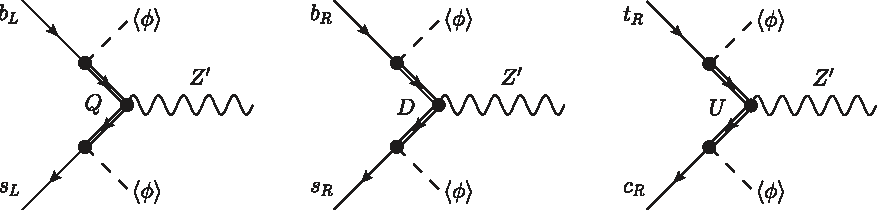
\includegraphics[width=\textwidth]{Bilder/NeueQuarks.pdf}
	\caption{Wechselwirkung von SM-Quarks mit dem Eichboson $Z'$}
\end{figure}}
\end{frame}

%\begin{frame}{Neue Wechselwirkung}
%\framesubtitle{Kopplung der neuen Quarks an die SM-Quarks}
%\begin{figure}
%	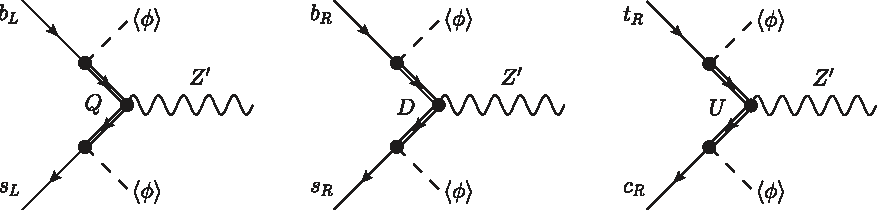
\includegraphics[width=\textwidth]{Bilder/NeueQuarks.pdf}
%	\caption{Wechselwirkung von SM-Quarks mit dem Eichboson $Z'$ (aus \cite{InColour})}
%\end{figure}
%\end{frame}


\begin{frame}{Erklärung seltener $B$-Zerfälle}
\vspace*{-.5cm}
\begin{columns}[c]
\begin{column}{.5\textwidth}
\begin{figure}
	\centering
	\resizebox{\textwidth}{!}{
	\begin{tikzpicture}
\tikzstyle{centerArrow}=[decoration={
	markings,
	mark=at position 0.5 with {\fill (2pt,0)--(-2pt,2.31pt)--(-2pt,-2.31pt)--cycle;}}]
\begin{scope}%[yshift=5cm]
\def\xmove{2.5}
\def\ymove{1.25}
\def\centerSize{0.18}

\node [fill, circle,inner sep=\centerSize cm] (tCenter) {};
\node (Left) at (-\xmove,0) {$b$};
\node (upperRight) at (\xmove,0.5*\ymove) {$s$};
\node (middleRight) at (\xmove,0) {$\mu$};
\node (lowerRight) at (\xmove,-0.5*\ymove) {$\bar{\mu}$};

\draw [centerArrow,postaction={decorate}]  (Left) -- (tCenter) ;
\draw [centerArrow,postaction={decorate}]  (tCenter) -- (upperRight) ;
\draw [centerArrow,postaction={decorate}]  (tCenter) -- (middleRight) ;
\draw [centerArrow,postaction={decorate}]  (lowerRight) -- (tCenter) ;

\node (indep1) at (-\xmove, \ymove) {$\bar{u},\bar{d},\bar{s}$};
\node (indep2) at (\xmove, \ymove) {$\bar{u},\bar{d},\bar{s}$};
\draw [centerArrow,postaction={decorate}] (indep2) -- (indep1);

\end{scope}
\end{tikzpicture}
	}
	\caption{$B\rightarrow K\mu\bar{\mu}$ bzw. $B_s\rightarrow \Phi\mu\bar{\mu}$}
\end{figure}
\end{column}
\begin{column}{.45\textwidth}
	\uncover<2->{
\begin{figure}
	\centering
	\resizebox{\textwidth}{!}{
		\begin{tikzpicture}
\tikzstyle{centerArrow}=[decoration={
	markings,
	mark=at position 0.5 with {\fill (2pt,0)--(-2pt,2.31pt)--(-2pt,-2.31pt)--cycle;}}]
\begin{scope}%[xshift=-8cm]
\def\xmove{2.5}
\def\ymove{0.5}
\def\centerSize{0.08}

\node [fill, circle, inner sep=\centerSize cm] (tCenter1)  {};
\coordinate (tCenter2) at (1,-1cm);
\node (Left) at (-\xmove,0) {$b$};
\node (upperRight) at (\xmove,0) {$s$};
\node (middleRight) at ([xshift=1.5cm,yshift=\ymove cm] tCenter2) {$\mu$};
\node (lowerRight) at ([xshift=1.5cm,yshift=-\ymove cm] tCenter2) {$\bar{\mu}$};


\draw [centerArrow,postaction={decorate}]  (Left) -- (tCenter1) ;
\draw [centerArrow,postaction={decorate}]  (tCenter1) -- (upperRight) ;
\draw [centerArrow,postaction={decorate}]  (tCenter2) -- (middleRight) ;
\draw [centerArrow,postaction={decorate}]  (lowerRight) -- (tCenter2) ;
\draw [decoration={snake, segment length=1.5mm, amplitude=0.5mm},decorate] (tCenter1) -- (tCenter2) ;
\end{scope}
\end{tikzpicture}
	}
	\caption{$b\rightarrow s\mu\bar{\mu}$}
\end{figure}}
\end{column}
\end{columns}
\uncover<3->{Beschreibung mit $Z'$-Austausch:
	\[ H = \frac{Y_{Qb}Y_{Qs}^*}{2m_Q^2}(\bar{s}_L\gamma_\mu b_L)(\bar{\mu}\gamma^\mu\mu)-\frac{Y_{Db}Y_{Ds}^*}{2m_D^2}(\bar{s}_R\gamma_\mu b_R)(\bar{\mu}\gamma^\mu\mu) \]}
\uncover<4->{Beschränkung der Masse auf:
\[ m_{Q,D} \approx \SI{25}{\tera\electronvolt}\sqrt{\text{Re}\left(Y_{(Q,D)b}Y_{(Q,D)s}\right)} \]}
\note{Alle anderen Parameter =0.}
\end{frame}


\begin{frame}{Loop-Diagramm zur Streuung am Atomkern}
\begin{columns}
\begin{column}{.35\textwidth}
%	\begin{figure}[H]
		\resizebox{\textwidth}{!}{
			\begin{tikzpicture}
\tikzstyle{centerArrow}=[decoration={
	markings,
	mark=at position 0.5 with {\fill (2pt,0)--(-2pt,2.31pt)--(-2pt,-2.31pt)--cycle;}}]

\begin{scope}[xshift=6cm,yshift=5cm]
\def\xmove{2}
\def\ymove{1.25}
\def\centerShift{2cm}
\def\centerCircle{1cm}
\def\centerSize{0.05cm}
\coordinate (tCenter1) at (0,0);
\coordinate (tCenter2) at (0,-\centerShift);
\coordinate (tCenter3) at (0,-\centerShift-\centerCircle);
\coordinate (tCenter4) at (0,-\centerShift-\centerCircle-\centerShift);

\node (upperLeft) at (-\xmove,\ymove) {$\chi$};
\node (upperRight) at (\xmove,\ymove) {$\chi$};
\node (lowerLeft) at (-\xmove,-\centerShift-\centerCircle-\centerShift-\ymove cm) {$N$};
\node (lowerRight) at (\xmove,-\centerShift-\centerCircle-\centerShift-\ymove cm) {$N$};

\draw [centerArrow,postaction={decorate}]  (upperLeft) -- (tCenter1) ;
\draw [centerArrow,postaction={decorate}]  (tCenter1) -- (upperRight) ;
\draw [centerArrow,postaction={decorate}]  (lowerLeft) -- (tCenter4) ;
\draw [centerArrow,postaction={decorate}]  (tCenter4) -- (lowerRight) ;
\draw [decoration={snake, segment length=1.5mm, amplitude=0.5mm},decorate] (tCenter1) -- (tCenter2) ;
\node at (0.5,-\centerShift/2) {$Z'$};
\draw [
        decoration={markings, mark=at position 0.5 with {\fill (2pt,0)--(-2pt,2.31pt)--(-2pt,-2.31pt)--cycle;}, mark=at position 1 with {\fill (2pt,0)--(-2pt,2.31pt)--(-2pt,-2.31pt)--cycle;}},
        postaction={decorate}
] ([yshift=.5cm]tCenter3) ellipse(.45 and 0.5);
\node at ([yshift=-\centerCircle/2,xshift=0.75cm]tCenter2) {$l$};
\node at ([yshift=-\centerCircle/2,xshift=-0.75cm]tCenter2) {$l$};
\draw [decoration={snake, segment length=1.5mm, amplitude=0.5mm},decorate] (tCenter3) -- (tCenter4) ;
\node at (0.5,-\centerShift/2-\centerCircle-\centerShift) {$\gamma$};
\end{scope}
\end{tikzpicture}
		}
		%		\captionsetup{width=\textwidth}
%		\caption{Loop-Wechselwirkung zur Streuung DM am Atomkern.}
%	\end{figure}
\end{column}
\begin{column}{.65\textwidth}
	Wirkungsquerschnitt ohne Impulsübertrag:
	\[ \sigma_\text{0,loop} = \frac{\mu_{A\chi}^2}{A^2\pi}\left(\frac{\alpha_{em}Z}{3\pi}\ \frac{g'^2q_\chi q_l}{m_{Z'}^2}\log\left(\frac{m_\mu^2}{m_\tau^2}\right)\right)^2 \]
\end{column}
\end{columns}
\end{frame}


\begin{frame}{Beschränkung der Parameter}
$B$-Zerfälle:
	\[ \SI{540}{\giga\electronvolt}\lessapprox\frac{m_{Z'}}{g'}\lessapprox\SI{4.9}{\tera\electronvolt} \]
Relic Density:
	\[ m_{Z'}\approx 2m_\chi \]
Direct Detection $(q_\chi=q_l=1)$:
	\[ \SI{10}{\giga\electronvolt}\lessapprox m_{Z'} \lessapprox\SI{46}{\giga\electronvolt} \]
	\[ \SI{2e-3}{}\lessapprox g' \lessapprox\SI{e-2}{} \]
\end{frame}
